\documentclass[11pt]{article}

\usepackage[utf8]{inputenc}
\usepackage[portuges]{babel}
\usepackage{indentfirst}
\usepackage{natbib}
\usepackage{graphicx}
\usepackage{geometry}
\usepackage[export]{adjustbox}
\usepackage[shortlabels]{enumitem}
\usepackage{minted}
\usepackage{makeidx}
\usepackage{newfloat}
\usepackage{lipsum}
\usepackage{enumitem}
\usepackage{multirow}
\usepackage{array}
\usepackage{caption}
\usepackage{underscore}

 \geometry{
    a4paper,
    total={130mm,227mm},
    left=40mm,
    top=40mm,
}
\addto\captionsportuges{
    \renewcommand*\contentsname{\LARGE Índice}}

\begin{document}

\begin{titlepage}
    \begin{center}
        
\includegraphics[width=0.4\textwidth]{Imagens/uni.png}
    
        \vspace{2cm}
        
        \textbf{\Huge Laboratórios de Informática III}\par

        \vspace{3cm}
        
        \large 
        
        Carlos Diogo Fernandes Pina A95349 \\
        Lara Beatriz Pinto Ferreira A95454 \\ 
        João Machado Gonçalves A97321 \\

        \vspace{2cm}
    
        \begin{figure}[hbt!]
        \minipage{0.3\textwidth}
            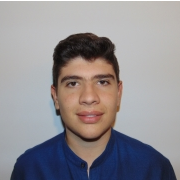
\includegraphics[width=\linewidth]{Imagens/febras.png}
            \centering
            \caption{A95349}
        \endminipage\hfill
        \minipage{0.3\textwidth}
            
\includegraphics[width=\linewidth]{Imagens/Photo (2).jpg}
            \centering
            \caption{A95454}
        \endminipage\hfill        
        \minipage{0.3\textwidth}
            
\includegraphics[width=\linewidth]{Imagens/slash.png}
            \centering
            \caption{A97321}
        \endminipage
        \end{figure}
        
        \vspace{3cm}
        \textbf{18 de Novembro de 2023}
    \end{center}
    

\end{titlepage}


\thispagestyle{empty}
\cleardoublepage
\tableofcontents 
\clearpage


\section {Introdução}´

    No âmbito da Unidade Curricular de Laboratórios de Informática III da licenciatura em Engenharia Informática, foi nos requisitado a implementação de um sistema em C que consiga dar resposta a \textit{queries} pedidas, sobre a dados fornecidos em formato de texto.
    Na primeira fase foi nos requisitado a implementação de um \textit{parser} em C que validasse as linhas dos quatro ficheiros \textit{.csv} (\textit{users}, \textit{flights}, \textit{passengers} e \textit{reservations}) que nos foram disponibilizados, assim como a implementação de pelo menos seis \textit{queries}, que no caso resolvemos implementar as \textit{queries 1,3,4,5,8,9}. 
    Nesta segunda e última fase, o objetivo era a implementação do modo interativo, dimensionar a solução para ficheiros de entrada com uma ordem de grandeza superior, completar totalmente as \textit{queries} requisitadas e testar e avaliar o tempo de execução dessas mesmas \textit{queries}.
    Para a realização do presente projeto, aplicamos os conhecimentos essenciais da linguagem C e Engenharia de Software, principalmente modularidade e encapsulamento.

\section{Arquitetura do sistema}

\begin{figure}[hbt!]
        \centering
        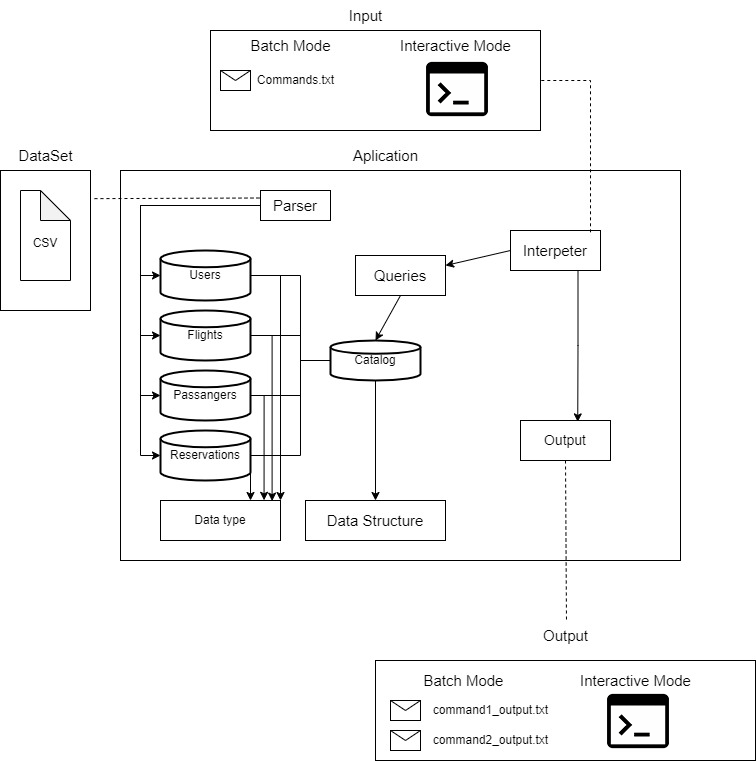
\includegraphics[width=0.7\textwidth]{Imagens/Estrutura.png}
        \caption{Arquitetura de Sistema}
        \label{fig:example}
    \end{figure}

\section{Estratégia utilizada}
    Após a análise do enunciado, decidimos adotar uma abordagem que envolve a criação de arquivos para armazenar dados válidos e a implementação de caches para otimizar os acessos a esses arquivos. Esta estratégia será aplicada às estruturas de dados \textit{users}, \textit{flights}, \textit{reservations} e \textit{passengers}, com a intenção de realizar operações iterativas de forma eficiente.
    \subsection{Estruturas de dados utilizadas para representar utilizadores, voos, reservas e passageiros}
    As estruturas de dados referidas foram criadas de forma a ser possível realizar, o mais eficientemente possível, tanto a nível de performance como de memória, as \textit{queries} que implementamos.

\subsubsection{Utilizadores}

   Após a criação da cache, fazemos o parsing,análise e validação da \textit{dataset},os \textit{users} válidos são guardados num \textit{file users_valid.csv}. Ao realizar uma pesquisa, a busca é primeiro realizada na cache antes de consultar o arquivo, utilizando o ID do usuário como chave. Essa abordagem visa otimizar a eficiência do processo, favorecendo o acesso rápido às informações mais recentes armazenadas em memória, antes de recorrer aos dados armazenados nos arquivos.
    Cada voo é representado no sistema pela \textit{struct Users}, com as seguintes características:
    
    \begin{figure}[hbt!]
        \centering
        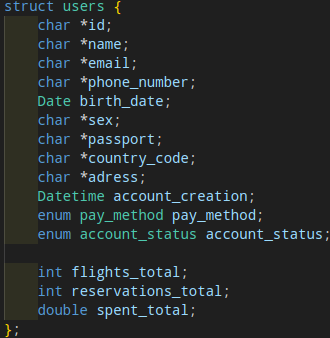
\includegraphics[width=0.5\textwidth]{Imagens/struct users.png}
        \caption{Struct Users}
        \label{fig:example}
    \end{figure}
    \newpage
     \begin{itemize}
                \item Id : O identificador do \textit{user} é representado como uma \textit{string}
                \item Name : O Nome do \textit{user} é representado como uma \textit{string}
                \item Email : O email do \textit{user} é representado como uma \textit{string}
                \item Phone_number : O número de telemóvel do \textit{user} é representado como uma \textit{string}
                \item Birth_date : A data de nascimento do \textit{user} é representada como um \textit{datetime}
                \item Sex : O género do \textit{user} é representado como uma \textit{string}
                \item Passaport : O número do passaporte do \textit{user} é presentado como uma \textit{string}
                \item Country_code : O código do país de residência
                \item Address : A morada do \textit{user} é representado como uma \textit{string}
                \item Account_creation : A data de criação da conta é representada com um \textit{datetime}
                \item Pay_method : O método de pagamento é representado como um \textit{enum} 
                \item Account_status : O estado da conta é representado como um \textit{enum} 
                \item Flights_total : O número de voos realizados pelo \textit{user} é representado como um inteiro
                \item Reservations_total : O número de reservas realizadas pelo \textit{user} é representado como um inteiro
                \item Spent_total : O total de dinheiro gasto pelo \textit{user} é representado como um \textit{double}
        \end{itemize}
\newpage
\subsubsection{Voos}

    Após a criação da cache, fazemos o parsing,análise e validação da \textit{dataset},as \textit{flights} válidos são guardados num \textit{file flights_valid.csv}. Ao realizar uma pesquisa, a busca é primeiro realizada na cache antes de consultar o arquivo, utilizando o ID do usuário como chave. Essa abordagem visa otimizar a eficiência do processo, favorecendo o acesso rápido às informações mais recentes armazenadas em memória, antes de recorrer aos dados armazenados nos arquivos.
    Cada voo é representado no sistema pela \textit{struct Flights}, com as seguintes características:

    \begin{figure}[hbt!]
        \centering
        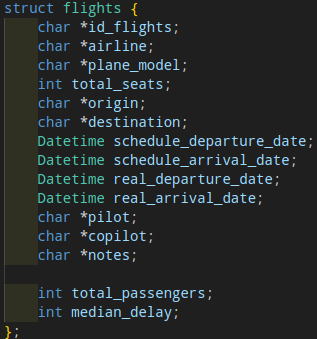
\includegraphics[width=0.5\textwidth]{Imagens/struct flights.png}
        \caption{Struct Flights}
        \label{fig:example}
    \end{figure}
    
     \begin{itemize}
        \item Id_flights : O identificador do \textit{Flight} é representado como uma \textit{string}
        \item Airline : A companhia aérea que realizou o \textit{Flight} é representada com uma \textit{string}
        \item Plane_model : O modelo do avião usado na \textit{Flight} é representada com uma \textit{string}
        \item Total_seats: O número de lugares total do avião usado na \textit{Flight} é representada como um inteiro
        \item Origin : O aeroporto de origem da \textit{Flight} é representada como uma \textit{string}
        \item Destination : O aeroporto de destino da \textit{Flight} é representada como uma \textit{string}
        \item Schedule_departure_date : A data e hora planeada para a partida da \textit{Flight} é representado por um \textit{datetime}
        \item Schedule_arrival_date :  A data e hora planeada para a chegada da \textit{Flight} é representado por um \textit{datetime}
        \item Real_departure_date : A data e hora efetiva da partida da \textit{Flight} é representado por um \textit{datetime} 
        \item Real_arrival_date : A data e hora efetiva da \textit{Flight} é representado por um \textit{datetime} 
        \item Pilot : O nomedo  piloto que realizou a \textit{Flight} é representado por uma \textit{string}
        \item Copilot : O nome do Co-piloto que realizou a \textit{Flight} é representado por uma \textit{string}
        \item Notes : As observações sobre a \textit{Flight} são representadas como uma \textit{string}
        \item num_passengers : O número de passageiros que realizou a \textit{Flight} é representado como um inteiro
        \item Delay : O atraso da \textit{flight}, em segundos, é representado como um inteiro
    \end{itemize}
\subsubsection{Reservas}

       Após a criação da cache, fazemos o parsing, análise e validação da \textit{dataset},as \textit{reservations} válidos são guardados num \textit{file reservations_valid.csv}. Ao realizar uma pesquisa, a busca é primeiro realizada na cache antes de consultar o arquivo, utilizando o ID do usuário como chave. Essa abordagem visa otimizar a eficiência do processo, favorecendo o acesso rápido às informações mais recentes armazenadas em memória, antes de recorrer aos dados armazenados nos arquivos.
    Cada voo é representado no sistema pela \textit{struct Reservations}, com as seguintes características:
    
    \begin{figure}[hbt!]
        \centering
        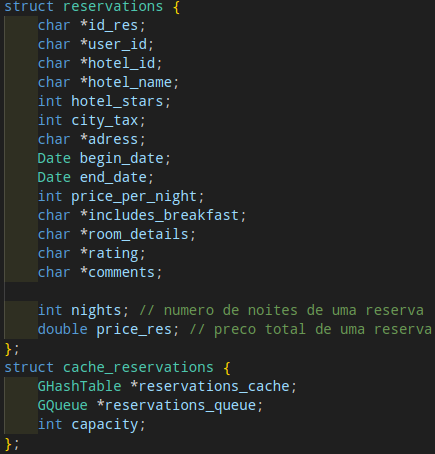
\includegraphics[width=0.6\textwidth]{Imagens/struct reservations.png}
        \caption{Struct Reservations}
        \label{fig:example}
    \end{figure}
    
    \newpage
    
     \begin{itemize}
        \item Id_res : O identificador da \textit{Reservation} é representado como uma \textit{string}
        \item User_id : O identificador do \textit{User} que fez a \textit{Reservation} é representado como uma \textit{string}
        \item Hotel_id : O identificador do hotel é representado como uma \textit{string}
        \item Hotel_name : O nome do hotel é representado como uma \textit{string}
        \item Hotel_stars : O número de estrelas do hotel é representado como um inteiro
        \item City_tax : A percentagem do imposto da cidade é representado como um inteiro
        \item Begin_date : A data de início da \textit{Reservation} é representado como uma \textit{date}
        \item End_date : A data de fim da \textit{Reservation} é representado como uma \textit{date}
        \item Price_per_night : O preço por noite é representado por um inteiro
        \item Includes_breakfast : A inclusão de pequeno-almoço na \textit{Reservation} é representa como uma \textit{string}
        \item Room_details : Os detalhes sobre o quarto são representado como uma \textit{string} 
        \item Rating : A classificação atribuída pelo \textit{user} é representada como uma \textit{string}
        \item Comment : O comentário sobre a reserva 
        \item Nights : O número de noites que abrangidas na \textit{Reservation} é representada como um inteiro
        \item Total_price : O preço total da \textit{Reservation} é representado como um \textit{double}
    \end{itemize}
\newpage
\subsubsection{Passageiros}

       Após a criação da cache, fazemos o parsing,análise e validação da \textit{dataset},os \textit{passengers} válidos são guardados num \textit{file passengers_valid.csv}. Ao realizar uma pesquisa, a busca é primeiro realizada na cache antes de consultar o arquivo, utilizando o ID do usuário como chave. Essa abordagem visa otimizar a eficiência do processo, favorecendo o acesso rápido às informações mais recentes armazenadas em memória, antes de recorrer aos dados armazenados nos arquivos.
    Cada voo é representado no sistema pela \textit{struct Flights}, com as seguintes características:
    
    \begin{figure}[hbt!]
        \centering
        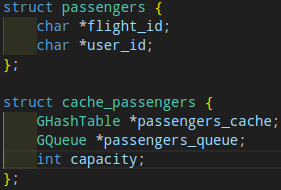
\includegraphics[width=0.6\textwidth]{Imagens/struct passengers.png}
        \caption{Struct Passengers}
        \label{fig:example}
    \end{figure}
    
    \begin{itemize}
        \item Flight_Id : O identificador da \textit{Flight} é representado como uma \textit{string}
        \item User_Id : O identificador do \textit{User} é representado como uma \textit{string}
    \end{itemize}
\newpage


\subsection{Estratégia de modularização e encapsulamento}

Mantivemos a modularização e encapsulamento,pois estes promovem uma maior organização, leitura e facilidade de manutenção do código, que por sua vez auxiliam no processo de desenvolvimento, desta forma decidimos implementar os seguintes módulos:
    \begin{itemize}
        \item Users : Representação de um \textit{User}, métodos de manipulação dos mesmos, a sua cache e metodos de manipulação da mesma
        \item Flights : Representação de um \textit{Flight}, métodos de manipulação dos mesmos, a sua cache e metodos de manipulação da mesma
        \item Reservations : Representação de um \textit{Reservation}, métodos de manipulação dos mesmos, a sua cache e metodos de manipulação da mesma
        \item Passengers : Representação de um \textit{Passenger}, métodos de manipulação dos mesmos, a sua cache e metodos de manipulação da mesma
        \item Catalog : Agregação dos diversos catalogos e estruturas
        \item Date : Representação de um \textit{Date} e/ou \textit{Datetime}
        \item Valid : Agregado de métodos de validação
        \item Prints : Agregado de métodos de output(Batch e Menu Interativo)
    \end{itemize}

\newpage

\section{Modo Interativo}
Como requesitado, nesta segunda fase, para além do modo batch, no qual o programa é executado com dois argumentos (sendo o primeiro o caminho para a pasta onde estão os ficheiros de entrada e o segundo o caminho para um ficheiro de texto que contém uma lista de comandos a serem executados), implementamos também um modo interativo que recebe input do utilizador e apresenta as respostas às queries pedidas no terminal, usando um método de paginação.

\section{Queries}


\subsection{Query 1}
\subsubsection{Descrição}
Listar o resumo de um utilizador, voo, ou reserva, consoante o identificador recebido por
argumento. É garantido que não existem identificadores repetidos entre as diferentes entidades. A
query deverá retornar as seguintes informações:
\begin{itemize}
        \item Utilizador : nome;sexo;idade;código_do_país;passaporte;número_voos;número_reservas;total_gasto
        \item Voo : companhia;avião;origem;destino;partida_est;chegada_est;número_passageiros;tempo_atraso
        \item Reserva : id_hotel;nome_hotel;estrelas_hotel;data_início;data_fim;pequeno_almoço;número_de_noites;preço_total
\end{itemize}
Não deverão ser retornadas informações para utilizadores com account_status = “inactive”.
    
\subsubsection{Implementação}
Se o identificador conter apenas dígitos, iremos procurar por uma \textit{flights}, caso contrário, se os primeiros 4 caracteres forem '\textit{Book}', procuraremos por uma \textit{reservations}, caso nenhuma das condições anteriores se verifique, procuramos por um \textit{users}.
Todas as pesquisas são inicialmente conduzidas na cache correspondente ao dado procurado, sendo apenas em seguida consultados os arquivos respectivos.
Em todos os casos é devolvida uma cópia dos valores encontrados ou nada se não existirem exceto no caso dos utilizadores com \textit{account_status = “inactive”} que também não devolve nada.
\subsection{Query 2}
\subsubsection{Descrição}
Listar os voos ou reservas de um utilizador, se o segundo argumento for flights ou reservations,
respetivamente, ordenados por data (da mais recente para a mais antiga). Caso não seja fornecido
um segundo argumento, apresentar voos e reservas, juntamente com o tipo (flight ou reservation).
Para os voos, date = schedule_departure_date (contudo, deverá ser descartada a componente das
horas/minutos/segundos no output), enquanto que para as reservas, date = begin_date.5 Em caso
de empate, ordenar pelo identificador (de forma crescente). Tal como na Q1, utilizadores com
account_status = “inactive” deverão ser ignorados.

    
\subsubsection{Implementação}

 

\newpage
\subsection{Query 3}
\subsubsection{Descrição}
Apresentar a classificação média de um hotel, a partir do seu identificador.

\subsubsection{Implementação}
Procuramos todas as \textit{reservations}, no arquivo das mesmas, que foram efetuadas no hotel com o identificador especificado e obtemos todas classificações. No fim, calculamos a media dessas classificações.

\subsection{Query 4}
\subsubsection{Descrição}
Listar as reservas de um hotel, ordenadas por data de início (da mais recente para a mais
antiga). Caso duas reservas tenham a mesma data, deve ser usado o identificador da reserva como
critério de desempate (de forma crescente).

\subsubsection{Implementação}

\newpage
\subsection{Query 5}
\subsubsection{Descrição}

Listar os voos com origem num dado aeroporto, entre duas datas, ordenados por data de partida
estimada (da mais recente para a mais antiga). Um voo está entre <begin_date> e <end_date> caso a
sua respetiva data estimada de partida esteja entre <begin_date> e <end_date> (ambos inclusivos).
Caso dois voos tenham a mesma data, o identificador do voo deverá ser usado como critério de
desempate (de forma crescente).


\subsubsection{Implementação}

\subsection{Query 6}
\subsubsection{Descrição}
Listar o top N aeroportos com mais passageiros, para um dado ano. Deverão ser contabilizados
os voos com a data estimada de partida nesse ano. Caso dois aeroportos tenham o mesmo valor,
deverá ser usado o nome do aeroporto como critério de desempate (de forma crescente).

    
\subsubsection{Implementação}

\subsection{Query 7}
\subsubsection{Descrição}
Listar o top N aeroportos com a maior mediana de atrasos. Atrasos num aeroporto são calculados a partir da diferença entre a data estimada e a data real de partida, para voos com origem nesse
aeroporto. O valor do atraso deverá ser apresentado em segundos. Caso dois aeroportos tenham
a mesma mediana, o nome do aeroporto deverá ser usado como critério de desempate (de forma
crescente).

    
\subsubsection{Implementação}

\subsection{Query 8}
\subsubsection{Descrição}

Apresentar a receita total de um hotel entre duas datas (inclusive), a partir do seu identificador.
As receitas de um hotel devem considerar apenas o preço por noite (price_per_night) de todas as
reservas com noites entre as duas datas. E.g., caso um hotel tenha apenas uma reserva de 100€/noite
de 2023/10/01 a 2023/10/10, e quisermos saber as receitas entre 2023/10/01 a 2023/10/02, deverá ser
retornado 200€ (duas noites). Por outro lado, caso a reserva seja entre 2023/10/01 a 2023/10/02,
deverá ser retornado 100€ (uma noite).

\newpage
\subsubsection{Implementação}
Ao receber como input o identificador do hotel e as datas de início e fim do período que queremos avaliar, a função verifica se as datas são válidas, de seguida procuramos todas as \textit{reservations}, no arquivo das mesmas, que foram efetuadas num hotel e período especificados, calculamos o preço de cada \textit{reservation} nesse período e somamos à receita total.


\subsection{Query 9}
\subsubsection{Descrição}

Listar todos os utilizadores cujo nome começa com o prefixo passado por argumento, ordenados
por nome (de forma crescente). Caso dois utilizadores tenham o mesmo nome, deverá ser usado
o seu identificador como critério de desempate (de forma crescente). Utilizadores inativos não
deverão ser considerados pela pesquisa

\subsubsection{Implementação}
Procuramos todos os \textit{users}, no arquivo dos mesmos, cujo nome começa com o prefixo especificado e a sua conta não está inativa, usamos-los para criar uma lista e organizamos essa mesma lista consoante os requisitos em cima.
\subsection{Query 10}
\subsubsection{Descrição}
Apresentar várias métricas gerais da aplicação. As métricas consideradas são: número de novos utilizadores registados (de acordo com o campo account_creation); número de voos (de acordo
com o campo schedule_departure_date); número de passageiros; número de passageiros únicos; e
número de reservas (de acordo com o campo begin_date). Caso a query seja executada sem argu-
mentos, apresentar os dados agregados por ano, para todos os anos que a aplicação tem registo.
Caso a query seja executada com um argumento, year, apresentar os dados desse ano agregados
por mês. Finalmente, caso a query seja executada com dois argumentos, year e month, apresentar
os dados desse ano e mês agregados por dia. O output deverá ser ordenado de forma crescente
consoante o ano/mês/dia

    
\subsubsection{Implementação}


\section{Teste de Performance}


\section{Conclusão}



\end{document}

